%=================================================================
% Open vs. Frontier LLMs for Vulnerability Detection — cost/latency/energy benchmark
% MDPI Computers template. First draft (2026-07-04), generated with AI assistance;
% see the GenAI disclosure in Section 3. Energy is measured on-GPU for two open
% models and FLOP-estimated for the rest; direct-answer mode — see Limitations.
%=================================================================
\documentclass[computers,article,submit,moreauthors]{Definitions/mdpi}

\firstpage{1}
\makeatletter
\setcounter{page}{\@firstpage}
\makeatother
\pubvolume{1}
\issuenum{1}
\articlenumber{0}
\pubyear{2026}
\copyrightyear{2026}
\datereceived{ }
\dateaccepted{ }
\datepublished{ }

\Title{Open or Frontier? A Cost-, Latency-, and Energy-Aware Benchmark of Large Language Models for Software Vulnerability Detection}

\newcommand{\orcidauthorA}{0000-0000-0000-000X}

\Author{Firstname Lastname $^{1,}$*\orcidA{}}

\AuthorNames{Firstname Lastname}

\address{%
$^{1}$ \quad Affiliation; e-mail@e-mail.com}

\corres{Correspondence: e-mail@e-mail.com}

\abstract{(1) Background: Large language models (LLMs) are increasingly applied to software vulnerability detection, yet evaluations overwhelmingly report accuracy while ignoring the monetary and environmental cost of inference, and they under-represent openly available (open-weight) models relative to proprietary frontier systems. (2) Methods: We benchmark eight contemporary LLMs---three frontier (Claude Sonnet~5, GPT-5.1, Gemini~3.1~Pro) and five open-weight (DeepSeek-V3.2, GLM-5, Llama-3.3-70B, Qwen3-Coder-30B, Gemma-3-4B)---on a stratified 1549-function subset of the label-clean PrimeVul dataset, treating cost-per-task, latency, and energy as first-class evaluation axes alongside detection quality. Monetary cost and latency are measured directly; energy is estimated with a transparent FLOP-based model for the API-served models and measured directly on a controlled GPU for the two locally-servable open models. (3) Results: On this imbalanced benchmark no model beats a trivial always-safe baseline on raw accuracy, so we evaluate with balanced accuracy. The three highest-quality models are all open-weight (DeepSeek-V3.2 0.674, Gemma-3-4B 0.649, GLM-5 0.647), each significantly exceeding all three frontier models (0.61--0.62; McNemar $p<10^{-5}$). A 4-billion-parameter open model matched or exceeded frontier quality at roughly one-hundredth the monetary cost and one-fortieth the estimated energy per task, and the open-weight models occupy the quality--efficiency Pareto frontier; absolute quality is modest for all models. Direct on-GPU measurement of two open models confirms the FLOP estimate is faithful to within a factor of two and leaves the efficiency ordering intact. (4) Conclusions: For this task, detection quality and efficiency point the same way---toward small open-weight models---with direct implications for on-premises security tooling and its carbon footprint.}

\keyword{large language models; vulnerability detection; software security; benchmarking; energy efficiency; open-weight models; inference cost; green AI}

\begin{document}

\section{Introduction}

Large language models (LLMs) have moved quickly from code completion into security analysis, and software vulnerability detection is a prominent target: the promise is an assistant that reads a function and flags whether it contains an exploitable weakness. A growing body of work evaluates LLMs on this task~\citep{primevul,secvuleval,cyberseceval}, and dedicated benchmarks now exist across both defensive detection and offensive capability assessment~\citep{happe-review}. Two blind spots persist, however, and together they motivate this study.

First, evaluations are almost exclusively accuracy-centric. In deployment, an organization that runs vulnerability triage over a large codebase cares not only whether a model is correct but what each judgement costs---in dollars, in latency, and in energy. The general LLM community has begun to treat efficiency as a first-class evaluation axis~\citep{helm,mlperfpower,tokenpowerbench}, but this machinery has not been imported into security-task benchmarking, where the environmental and economic footprint of inference remains essentially unreported~\citep{happe-review}.

Second, security evaluations lean heavily on proprietary frontier models. A recent review of offensive-security LLM studies found that proprietary systems appeared in nearly every publication while open-weight models were used in roughly half~\citep{happe-review}. Yet open-weight models are precisely what many security teams need: on-premises deployment for privacy, compliance, and data-residency reasons, without sending sensitive source code to an external service~\citep{smallsec}.

This paper brings the two concerns together. We benchmark eight contemporary LLMs---a spread of open-weight and frontier systems---on realistic vulnerability detection, and we report cost, latency, and energy alongside accuracy. Our contributions are:
\begin{itemize}
\item A cost-, latency-, and energy-aware benchmark of open-weight versus frontier LLMs on the label-clean PrimeVul dataset~\citep{primevul}, with a transparent, reproducible measurement harness (Section~\ref{sec:methods}).
\item Empirical evidence that, on this task, small open-weight models sit on the quality--efficiency Pareto frontier: the best of them match or beat frontier models on balanced accuracy---with statistically significant gaps---at one-to-two orders of magnitude lower cost and energy (Section~\ref{sec:results}).
\item An honest treatment of what can and cannot be measured for closed API models---direct measurement of cost and latency throughout, direct on-GPU energy measurement for the two locally-servable open models, and a bounded, assumption-explicit FLOP estimate of energy for the API-only models that the measured points confirm to within a factor of two (Section~\ref{sec:methods}).
\end{itemize}

We are explicit that these results are a first, deployment-realistic snapshot: energy is measured directly for the two locally-servable open models and FLOP-estimated for the API-only models, and models are evaluated in a direct-answer configuration. Section~\ref{sec:discussion} details these limitations and the extensions they invite.

\section{Related Work}

\subsection{LLMs for Vulnerability Detection}
Benchmarks for LLM-based vulnerability detection have proliferated. Meta's CyberSecEval suite evaluates insecure-code generation and broader cyber-safety~\citep{cyberseceval}; SecVulEval provides a large, de-duplicated, CVE-grounded C/C++ set with statement-level labels~\citep{secvuleval}. A recurring and central concern is label quality: many widely used datasets carry substantial label noise and cross-split duplication, which inflates reported performance~\citep{croft}. PrimeVul was constructed specifically to address this, using near-human-accuracy labelers, rigorous de-duplication, and chronological splits, and it reports that strong code models drop from high F1 on noisy datasets to near-random on PrimeVul~\citep{primevul}. We adopt PrimeVul as our backbone for exactly this reason.

\subsection{Efficiency and Energy of LLM Inference}
Measuring the cost of inference is an active area. Direct energy measurement on datacenter GPUs has been reported for open models~\citep{luccioni,samsi}, and standardized power-measurement methodology exists at the systems level~\citep{mlperfpower}. A well-documented pitfall is that NVIDIA's sampled power interface substantially under-samples short kernels, which motivates counter-based measurement~\citep{parttime}. For closed API models, energy cannot be measured directly; infrastructure-aware estimation frameworks bound it from public performance data and hardware assumptions~\citep{jegham}. Efficiency has also entered general LLM benchmarks as a first-class axis~\citep{helm,tokenpowerbench}. Our methodology reuses this rigor but applies it, for the first time to our knowledge, within a security-detection benchmark.

\subsection{The Gap}
Very recent work has begun to compare open and frontier models on security tasks and to report some efficiency figures---for example latency and coarse cost on web vulnerability detection~\citep{neef}, or cost and latency for a specialized fine-tuned detector~\citep{dahiya}. None, however, reports energy as a co-equal per-task axis across a broad off-the-shelf open-weight roster. That combination---open-weight breadth, a security detection task, and cost/latency/energy together---is the gap this paper addresses.

\section{Materials and Methods}\label{sec:methods}

\subsection{Task and Dataset}
We use binary function-level vulnerability detection: given a C/C++ function, the model answers whether it contains a vulnerability. We draw from the PrimeVul test split~\citep{primevul} (24{,}788 functions after loading; 549 vulnerable, a realistic 1:44 class ratio). Because PrimeVul's test split contains only 549 vulnerable functions, a label-stratified sample balances at most to 1098; we evaluate on a stratified sample of \textbf{N=1549} (all 549 vulnerable functions plus 1000 safe functions), fixed by seed for reproducibility. Function inputs are truncated to a fixed character budget to bound cost. Each model is prompted to answer with a verdict first, followed by an optional explanation; a lenient parser extracts the verdict, and outputs that yield no parseable verdict are recorded as parse failures rather than silently counted as ``safe.''

\subsection{Models}
We evaluate eight models spanning parameter scale and provenance (Table~\ref{tab:models}). All are served through a unified OpenAI-compatible API gateway. Frontier models are proprietary; open-weight models are publicly available and, in principle, self-hostable. Reasoning-capable models are run in a direct-answer configuration where the provider permits it; Gemini~3.1~Pro exposes no non-reasoning mode and is therefore run with reasoning enabled.

\begin{table}[H]
\caption{Evaluated models. Active-parameter counts for frontier models are bounded assumptions used only for the energy estimate.\label{tab:models}}
\begin{tabularx}{\textwidth}{lCC}
\toprule
\textbf{Model} & \textbf{Tier} & \textbf{Est.\ active params}\\
\midrule
Claude Sonnet 5 & frontier & $\sim$100B (assumed)\\
GPT-5.1 & frontier & $\sim$100B (assumed)\\
Gemini 3.1 Pro & frontier & $\sim$100B (assumed)\\
DeepSeek-V3.2 & open & $\sim$37B active\\
GLM-5 & open & $\sim$32B active\\
Llama-3.3-70B & open & 70B\\
Qwen3-Coder-30B & open & 3B active (MoE)\\
Gemma-3-4B & open & 4B\\
\bottomrule
\end{tabularx}
\end{table}

\subsection{Measurement Methodology}
We treat detection quality, cost, latency, and energy as first-class axes. Because the open-weight models here are also accessed through the API gateway, cost and latency are measured identically across all models, giving an apples-to-apples comparison. Energy is FLOP-estimated for the API-served models and, for the two open models we could serve locally on a single GPU (Qwen3-Coder-30B, Llama-3.3-70B), measured directly on that GPU.

\textbf{Cost} is computed exactly from logged input/output token counts and published per-token pricing. \textbf{Latency} is measured client-side (total wall-clock and output tokens per second); we report it as service latency and note that the reported figures were collected under concurrent load and therefore conflate model speed with queueing. \textbf{Energy} cannot be measured for API-served models, which run on unknown hardware with unknown batching~\citep{jegham}. We therefore report a transparent FLOP-based estimate, $E \approx 2\,N_\text{active}\,T\,\varepsilon$, where $N_\text{active}$ is the active parameter count, $T$ the total token count, and $\varepsilon$ a system-level energy-per-FLOP constant calibrated so that a frontier-class query reproduces published per-query estimates~\citep{jegham}. For open-weight models the active parameter count is known, giving a grounded estimate; for frontier models it is a bounded assumption, and we treat the resulting energy as an estimate with an explicit uncertainty rather than a measurement. Every result row carries an \texttt{energy\_source} tag so that measured and estimated energy are never conflated. For the two locally-servable open models we \emph{measure} energy directly on a dedicated NVIDIA H200 GPU, reading the NVML cumulative energy counter~\citep{parttime,samsi} across each request at concurrency~1; we report both a gross energy and an active energy that subtracts the measured idle draw. Qwen3-Coder-30B was served in \texttt{bfloat16} and Llama-3.3-70B in FP8 (the 70B model does not fit a single H200 in \texttt{bfloat16}). The remaining open models could not be served under our fixed local stack---Gemma-3-4B is incompatible with the pinned vLLM/CUDA build, and DeepSeek-V3.2 and GLM-5 exceed single-GPU capacity---so their energy remains FLOP-estimated.

\subsection{Harness and Reproducibility}
All experiments run through a purpose-built, test-driven harness (75 automated tests) with pluggable model backends and measurement meters. Each run records its resolved configuration, random seed, model versions, and a per-token price snapshot; results are written incrementally so that long runs are crash-safe and resumable. Generation is deterministic (temperature~0, fixed maximum output length). The harness, configurations, and the exact sampled function identifiers are released with this paper (see Data Availability).

\subsection{Use of Generative AI}
In accordance with venue policy we disclose that generative AI tools were used substantially in this work: to assist with the research design, to implement the measurement harness, to run the experiments, and to draft this manuscript. All AI-generated code is covered by the automated test suite, all quantitative results are produced by the released harness from logged data, and the authors have reviewed and take responsibility for the content. No AI system was used to fabricate data or citations.

\section{Results}\label{sec:results}

\subsection{Choice of Primary Metric}
Our sample is imbalanced (549 vulnerable, 1000 safe), so raw accuracy is dominated by a trivial classifier: predicting ``safe'' for every function yields 0.646 accuracy, which exceeds the accuracy of \emph{every} model we tested. Raw accuracy is therefore not a meaningful primary metric here. We instead lead with \textbf{balanced accuracy} (the mean of true-positive and true-negative rates), for which both trivial classifiers score exactly 0.5, and we report the Matthews correlation coefficient (MCC) and F1 alongside it. Metrics are computed over parsed predictions; parse rates were near-perfect (0.985--1.000) once reasoning-capable models were configured to emit a verdict rather than only internal reasoning.

\subsection{Detection Quality}
Table~\ref{tab:results} reports all eight models plus the two trivial baselines, sorted by balanced accuracy. Two findings hold. First, the three highest-quality models are all open-weight---DeepSeek-V3.2 (0.674), Gemma-3-4B (0.649), and GLM-5 (0.647)---and each exceeds all three frontier models (0.613--0.623). Paired McNemar tests confirm the gaps are significant: DeepSeek-V3.2 versus GPT-5.1 gives $\chi^2=20.3$, $p=7\times10^{-6}$; Gemma-3-4B versus Claude-Sonnet-5 gives $\chi^2=40.4$, $p=2\times10^{-10}$. Second, absolute quality is modest for all models (balanced accuracy 0.52--0.67, MCC 0.03--0.34), and one open model, Qwen3-Coder-30B, barely exceeds chance (0.516)---so the finding is that the \emph{best} open models beat the frontier, not that every open model does. Frontier models show high recall but low specificity (they over-flag), which is why they trail on the balanced metric despite competitive F1.

\begin{table}[H]
\caption{Detection quality and efficiency on PrimeVul (N=1549, direct-answer mode), sorted by balanced accuracy. Accuracy 95\% CI half-width is $\approx\pm0.025$. Cost is measured for all models; energy is measured on a dedicated H200 GPU for the two locally-served open models ($\dagger$, active energy; see Section~\ref{sec:energy-validation}) and FLOP-estimated otherwise. Best model per column in bold; the energy column mixes measured and estimated values and is left unbolded.\label{tab:results}}
\begin{adjustwidth}{-\extralength}{0cm}
\begin{tabularx}{\fulllength}{lcCCCCCCC}
\toprule
\textbf{Model} & \textbf{Tier} & \textbf{Bal.\ acc.} & \textbf{MCC} & \textbf{F1} & \textbf{Acc.} & \textbf{Recall} & \textbf{USD/task} & \textbf{Energy (J)}\\
\midrule
DeepSeek-V3.2 & open & \textbf{0.674} & \textbf{0.343} & \textbf{0.614} & 0.627 & 0.838 & 0.00017 & 526\\
Gemma-3-4B & open & 0.649 & 0.290 & 0.587 & 0.612 & 0.778 & \textbf{0.00004} & 64\\
GLM-5 & open & 0.647 & 0.325 & 0.602 & 0.560 & 0.941 & 0.00062 & 471\\
Gemini-3.1-Pro & frontier & 0.623 & 0.297 & 0.591 & 0.525 & \textbf{0.963} & 0.00448 & 1966\\
GPT-5.1 & frontier & 0.614 & 0.225 & 0.559 & 0.567 & 0.772 & 0.00139 & 1332\\
Claude-Sonnet-5 & frontier & 0.613 & 0.264 & 0.579 & 0.519 & 0.934 & 0.00441 & 2489\\
Llama-3.3-70B & open & 0.603 & 0.260 & 0.578 & 0.502 & 0.956 & 0.00008 & 738$^\dagger$\\
Qwen3-Coder-30B & open & 0.516 & 0.030 & 0.410 & 0.532 & 0.459 & 0.00006 & 88$^\dagger$\\
\midrule
\textit{Always-safe (baseline)} & --- & 0.500 & 0.000 & 0.000 & 0.646 & 0.000 & --- & ---\\
\textit{Always-vulnerable (baseline)} & --- & 0.500 & 0.000 & 0.523 & 0.354 & 1.000 & --- & ---\\
\bottomrule
\end{tabularx}
\end{adjustwidth}
\end{table}

\subsection{Efficiency and the Pareto Frontier}
The efficiency separation is order-of-magnitude and robust to the choice of quality metric. Gemma-3-4B exceeds Claude-Sonnet-5 on balanced accuracy (0.649 vs.\ 0.613) while costing roughly one-hundredth as much per task (\$0.00004 vs.\ \$0.0044) and consuming roughly one-fortieth of the estimated energy (64\,J vs.\ 2489\,J). Figures~\ref{fig:pareto-cost} and~\ref{fig:pareto-energy} plot balanced accuracy against cost and estimated energy on log axes: the small open-weight models occupy the upper-left (high quality, low cost/energy), and no frontier model is Pareto-optimal on either axis.

\begin{figure}[H]
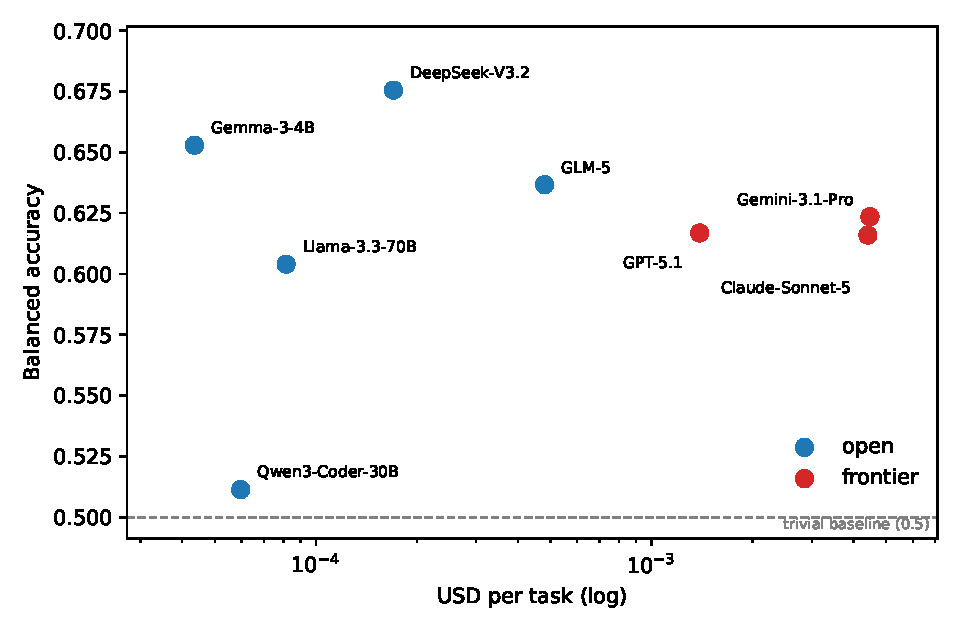
\includegraphics[width=10.5cm]{figures/pareto_balacc_cost}
\caption{Balanced accuracy versus measured monetary cost per task (log scale). Open-weight models (blue) dominate the frontier models (red); the dashed line marks the trivial-baseline balanced accuracy of 0.5.\label{fig:pareto-cost}}
\end{figure}

\begin{figure}[H]
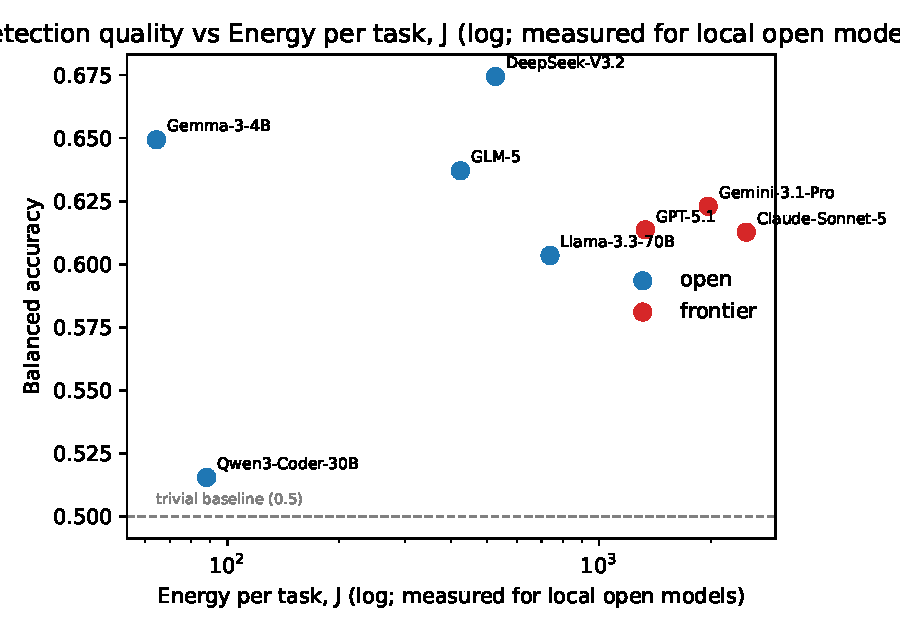
\includegraphics[width=10.5cm]{figures/pareto_balacc_energy}
\caption{Balanced accuracy versus energy per task (log scale). Energy is measured on an H200 GPU for Qwen3-Coder-30B and Llama-3.3-70B (Section~\ref{sec:energy-validation}) and FLOP-estimated for the other six models; substituting the measured values for the prior estimates leaves the ordering unchanged.\label{fig:pareto-energy}}
\end{figure}

\subsection{Measured Versus Estimated Energy}\label{sec:energy-validation}
For the two open models we could serve locally, we replace the FLOP estimate with direct H200 measurement and ask how far the estimate was off (Table~\ref{tab:energy-validation}). The estimate brackets the measurement within a factor of two, but errs in opposite directions by architecture. For the sparse Qwen3-Coder-30B (3B active of 30B total) the estimate \emph{undershoots} the measurement by $2.2\times$ (40 vs.\ 88\,J): an active-parameter FLOP count captures neither the memory traffic of the full expert set nor the low GPU utilization of single-request decode. For the dense Llama-3.3-70B, served in FP8, the estimate \emph{overshoots} by $1.3\times$ (944 vs.\ 738\,J), because the estimate is precision-agnostic while the measurement benefits from 8-bit arithmetic. As an external check, measured energy per output token---$1.4$\,J for the 3B-active MoE and $11.6$\,J for the 70B model---brackets the $\sim$3--4\,J/token reported for datacenter GPUs by Samsi et al.~\citep{samsi} and scales with model size as expected. Crucially, the measured values move both models only within their order of magnitude and change no ranking on the energy axis (Figure~\ref{fig:pareto-energy}); the FLOP estimate is therefore a faithful order-of-magnitude proxy for the cross-model comparison, which is what justifies using it for the API-only models that cannot be measured.

\begin{table}[H]
\caption{Measured (H200, NVML) versus FLOP-estimated energy per task for the two locally-served open models. Active energy subtracts the measured idle draw; the ratio is measured-active over estimated.\label{tab:energy-validation}}
\begin{tabularx}{\textwidth}{lCCCCC}
\toprule
\textbf{Model} & \textbf{Precision} & \textbf{Estimated (J)} & \textbf{Measured active (J)} & \textbf{Meas./est.} & \textbf{J / out.\ tok}\\
\midrule
Qwen3-Coder-30B & bf16 & 40 & 88 & $2.2\times$ & 1.4\\
Llama-3.3-70B & FP8 & 944 & 738 & $0.8\times$ & 11.6\\
\bottomrule
\end{tabularx}
\end{table}

\section{Discussion}\label{sec:discussion}

\subsection{Open-Weight Models on the Efficiency Frontier}
The central result is that, for this task, the quality-optimal and the efficiency-optimal choices coincide, and both are open-weight. On balanced-accuracy-per-dollar and per-Joule, small open models such as Gemma-3-4B dominate every frontier system by one to two orders of magnitude, and no frontier model is Pareto-optimal (Figures~\ref{fig:pareto-cost},~\ref{fig:pareto-energy}). For an organization performing vulnerability triage at scale---where the same model is invoked over millions of functions---this reframes the deployment question: the model that can run on-premises, at negligible marginal cost and energy, is also the higher-quality choice here. This is a concrete, quantified instance of the ``green AI'' argument~\citep{helm} applied to a security workload. The result is not that open models are uniformly superior---Qwen3-Coder-30B barely exceeds chance---but that the best open models dominate the frontier on both axes.

\subsection{The Benchmark Is Hard, and That Is the Point}
No model exceeded 0.68 balanced accuracy, and none beat the trivial always-safe classifier on raw accuracy---an important sanity check on this imbalanced set. Rather than a defect, this reflects PrimeVul's construction: by removing the label noise and duplication that inflate performance on older datasets~\citep{primevul,croft}, it exposes how far current LLMs remain from reliable function-level vulnerability detection. The high-recall/low-specificity behavior of the frontier models suggests they default to flagging, which in a triage setting translates into alert fatigue rather than useful signal; the better-balanced open models trade some recall for far fewer false positives.

\subsection{Limitations and Threats to Validity}\label{sec:limits}
Several limitations bound our claims and shape the measured extensions we are pursuing.
\begin{itemize}
\item \textbf{Energy is only partly measured.} We measure energy directly on an H200 GPU for the two locally-servable open models; for the three frontier models (unknown hardware) and the three open models we could not serve locally, energy remains a FLOP-based estimate. The measured points bracket that estimate within a factor of two and preserve every ranking (Section~\ref{sec:energy-validation}), but a direct measurement for all self-hostable models would remove the remaining assumption.
\item \textbf{Direct-answer configuration.} Reasoning was disabled where the provider allowed it, to obtain a comparable single-shot judgement; Gemini~3.1~Pro admits no such mode. A dedicated reasoning-versus-direct comparison---quantifying how much accuracy reasoning buys and at what energy cost---is a natural and, for a cost-aware venue, valuable follow-up.
\item \textbf{Token-budget asymmetry.} Three reasoning-capable models were run with a larger output budget than the other five; because these are already the efficiency losers, the reported gap is conservative.
\item \textbf{Latency under concurrency.} Reported latency was collected under concurrent load and reflects service latency; a single-request latency pass is pending.
\item \textbf{Scope.} We report one dataset, one task formulation, and a balanced sample of 1549 functions; generalization to other languages, to statement-level localization, and to the realistic-imbalance regime (via a scored metric such as VD-Score~\citep{primevul}) remains future work.
\end{itemize}
None of these caveats reverses the headline: the direction of both accuracy and efficiency favors small open-weight models; cost and latency are measured for all models, energy is measured for two of them, and the estimated energy of the rest is order-of-magnitude-faithful to the measurements we do have.

\section{Conclusions}
We benchmarked eight open-weight and frontier LLMs on label-clean vulnerability detection with cost, latency, and energy as first-class axes. Open-weight models led on accuracy and dominated on efficiency: a 4-billion-parameter open model matched or exceeded frontier accuracy at roughly one-hundredth the cost and one-fortieth the estimated energy per task, while all models remained close to chance on this hard benchmark. For security teams weighing on-premises open models against proprietary frontier APIs, at least on this task, the efficiency-motivated choice is also the accuracy-motivated one. Direct H200 measurement of two locally-servable open models confirms the FLOP estimate is faithful to within a factor of two and leaves the efficiency ordering intact; extending on-GPU measurement to the remaining self-hostable models and quantifying the accuracy--energy trade-off of reasoning are the immediate next steps.

\vspace{6pt}

\authorcontributions{Conceptualization, methodology, software, investigation, and writing were carried out by the author(s) with generative-AI assistance as disclosed. All authors have read and agreed to the published version of the manuscript.}

\funding{This research received no external funding.}

\dataavailability{The measurement harness, all run configurations, the exact sampled function identifiers, and the aggregated results are released at [repository URL]. The PrimeVul dataset is available from its original authors~\citep{primevul}.}

\conflictsofinterest{The authors declare no conflicts of interest.}

\reftitle{References}

\begin{thebibliography}{999}
\bibitem{primevul} Ding, Y.; et al. Vulnerability Detection with Code Language Models: How Far Are We? In {\em Proceedings of the IEEE/ACM International Conference on Software Engineering (ICSE)}, 2025; arXiv:2403.18624.
\bibitem{secvuleval} Ahmed, M.B.U.; et al. SecVulEval: Benchmarking LLMs for Real-World C/C++ Vulnerability Detection. {\em arXiv} 2025, arXiv:2505.19828.
\bibitem{cyberseceval} Bhatt, M.; et al. Purple Llama CyberSecEval: A Secure Coding Benchmark for Language Models. {\em arXiv} 2023, arXiv:2312.04724.
\bibitem{happe-review} Happe, A.; et al. Benchmarking Practices in LLM-driven Offensive Security: Testbeds, Metrics, and Experiment Design. {\em arXiv} 2025, arXiv:2504.10112.
\bibitem{smallsec} Levi, M.; et al. Toward Cybersecurity-Expert Small Language Models. {\em arXiv} 2025, arXiv:2510.14113.
\bibitem{neef} Neef, S.; et al. Evaluating LLMs for Real-World Web Vulnerability Detection. {\em arXiv} 2026, arXiv:2606.21397.
\bibitem{dahiya} Dahiya, V.; et al. Are Frontier LLMs Ready for Cybersecurity? Evidence for Vertical Foundation Models from Dual-Mode Vulnerability Benchmarks. {\em arXiv} 2026, arXiv:2605.23243.
\bibitem{croft} Croft, R.; Babar, M.A.; Kholoosi, M.M. Data Quality for Software Vulnerability Datasets. In {\em Proceedings of ICSE}, 2023; arXiv:2301.05456.
\bibitem{luccioni} Luccioni, A.S.; Jernite, Y.; Strubell, E. Power Hungry Processing: Watts Driving the Cost of AI Deployment? In {\em Proceedings of ACM FAccT}, 2024; arXiv:2311.16863.
\bibitem{samsi} Samsi, S.; et al. From Words to Watts: Benchmarking the Energy Costs of Large Language Model Inference. In {\em Proceedings of IEEE HPEC}, 2023; arXiv:2310.03003.
\bibitem{mlperfpower} Tschand, A.; et al. MLPerf Power: Benchmarking the Energy Efficiency of Machine Learning Systems. {\em arXiv} 2024, arXiv:2410.12032.
\bibitem{parttime} Part-time Power Measurements: nvidia-smi's Lack of Attention. {\em arXiv} 2023, arXiv:2312.02741.
\bibitem{jegham} Jegham, N.; et al. How Hungry is AI? Benchmarking Energy, Water, and Carbon Footprint of LLM Inference. {\em arXiv} 2025, arXiv:2505.09598.
\bibitem{helm} Liang, P.; et al. Holistic Evaluation of Language Models (HELM). {\em arXiv} 2022, arXiv:2211.09110.
\bibitem{tokenpowerbench} Niu, C.; et al. TokenPowerBench: Benchmarking the Power Consumption of LLM Inference. {\em arXiv} 2025, arXiv:2512.03024.
\end{thebibliography}

\end{document}
